%
% This is the LaTeX template file for lecture notes for CS294-8,
% Computational Biology for Computer Scientists.  When preparing
% LaTeX notes for this class, please use this template.
%
% To familiarize yourself with this template, the body contains
% some examples of its use.  Look them over.  Then you can
% run LaTeX on this file.  After you have LaTeXed this file then
% you can look over the result either by printing it out with
% dvips or using xdvi.
%
% This template is based on the template for Prof. Sinclair's CS 270.

\documentclass[11pt]{article}
\usepackage{charter}
\usepackage{graphicx}
\usepackage{url}
\usepackage{hyperref}
\usepackage{amsmath,amsthm,amssymb}
\usepackage{enumitem}

\setlength{\oddsidemargin}{0 in}
\setlength{\evensidemargin}{0 in}
\setlength{\topmargin}{-0.6 in}
\setlength{\textwidth}{6.5 in}
\setlength{\textheight}{8.5 in}
\setlength{\headsep}{0.75 in}
\setlength{\parindent}{0 in}
\setlength{\parskip}{0.1 in}

\newcommand{\PP}{\mathbb{P}}

%
% The following commands set up the lecnum (lecture number)
% counter and make various numbering schemes work relative
% to the lecture number.
%
\newcounter{lecnum}
\renewcommand{\thepage}{\thelecnum-\arabic{page}}
\renewcommand{\thesection}{\thelecnum.\arabic{section}}
\renewcommand{\theequation}{\thelecnum.\arabic{equation}}
\renewcommand{\thefigure}{\thelecnum.\arabic{figure}}
\renewcommand{\thetable}{\thelecnum.\arabic{table}}

%
% The following macro is used to generate the header.
%
\newcommand{\lecture}[5]{
   \pagestyle{myheadings}
   \thispagestyle{plain}
   \newpage
   \setcounter{lecnum}{#5}
   \setcounter{page}{1}
   \noindent
   \begin{center}
   \framebox{
      \vbox{\vspace{2mm}
    \hbox to 6.28in { {\bf Masters Bridge Program
                        \hfill Summer 2021} }
       \vspace{4mm}
       \hbox to 6.28in { {\Large \hfill Session {#1}: #2  \hfill} }
       \vspace{2mm}
       \hbox to 6.28in { {\it Instructor: #3 \hfill Contact: #4} }
      \vspace{2mm}}
   }
   \end{center}
   \markboth{Session #1: #2}{Session #1: #2}
   \vspace*{4mm}
}


%Use this command for a figure; it puts a figure in wherever you want it.
%usage: \fig{NUMBER}{SPACE-IN-INCHES}{CAPTION}
\newcommand{\fig}[3]{
			\vspace{#2}
			\begin{center}
			Figure \thelecnum.#1:~#3
			\end{center}
	}
% Use these for theorems, lemmas, proofs, etc.
\newtheorem{theorem}{Theorem}[lecnum]
\newtheorem{lemma}[theorem]{Lemma}
\newtheorem{fact}[theorem]{Fact}
\newtheorem{proposition}[theorem]{Proposition}
\newtheorem{claim}[theorem]{Claim}
\newtheorem{corollary}[theorem]{Corollary}
\theoremstyle{definition}
\newtheorem{definition}[theorem]{Definition}
\newtheorem{remark}[theorem]{Remark}
\newtheorem{example}[theorem]{Example}
\newtheorem{exercise}[]{Exercise}
\newenvironment{proofof}[1]{{\em Proof of #1.}}{\hfill%\rule{2mm}{2mm}
\qed}

% **** IF YOU WANT TO DEFINE ADDITIONAL MACROS FOR YOURSELF, PUT THEM HERE:
\renewcommand{\P}{\mathbb{P}}
\newcommand{\Z}{\mathbb{Z}}
\newcommand{\N}{\mathbb{N}}
\renewcommand{\H}{\mathcal{H}}
\renewcommand{\S}{\mathcal{S}}
\newcommand{\C}{\mathbb{C}}
\newcommand{\MAP}{\mathrm{MAP}}
\newcommand{\z}{\mathbf{z}}
\newcommand{\e}{\mathbf{e}}
\newcommand{\w}{\mathbf{w}}
\newcommand{\x}{\mathbf{x}}
\newcommand{\Rp}{\mathbb{R}_{>0}}
\newcommand{\im}{\mathrm{Im}}
\newcommand{\sign}{\mathrm{sign}}
\newcommand{\E}{\mathbb{E}}
\newcommand{\V}{\text{Var}}
\newcommand{\FF}{\mathcal{F}}
\newcommand{\R}{\mathbb{R}}
\newcommand{\lbr}{\langle}
\newcommand{\rbr}{\rangle}
\newcommand{\indi}{\mathds{1}}

\begin{document}
\lecture{3}{Convergence theorems}{Bryan Liu}{runjing\_liu@berkeley.edu}{3}

{\bf Supplemental reading}: Pitman, \textit{Probability} Chapters 2, 3.3

\section{The law of large numbers}

We go out in the world and collect data.
In a simplistic model of the world,
let the observed datapoints be denoted $X_1, ..., X_n$,
and we view the data as coming from random draws
of a distribution $F$.
In addition, if each data point is drawn
independently from all others, then we
say $X_1, ..., X_n$ are drawn \textit{i.i.d.} from $F$;
here, ``i.i.d." stands for \textit{independently and identically distributed}. Compactly, we write
\begin{align*}
  X_1, ..., X_n \stackrel{iid}{\sim} F.
\end{align*}

In most applications, the distribution $F$ is unknown.
The job of the statistician is to use the data
in order to estimate some properties
of the distribution $F$.
For example, we might be interested in the
mean of the distribution $F$,
and we could estimate the unknown mean of $F$ with the
sample mean
$\bar X_n = (1/n)\sum_{i=1}^n X_i$.

Why is this a good estimate?

\fbox{\begin{minipage}{\textwidth}
{\bf The law of averages}. Suppose $X_1, ..., X_n \stackrel{iid}{\sim} F$.
Let $\mu = \E(X_1)$ be the mean of the distribution $F$.
Define the sample mean
\begin{align*}
  \bar X_n = \frac{1}{n}\sum_{i=1}^n X_i.
\end{align*}

Then for any $\epsilon > 0$,
\begin{align}
  \P(|\bar X_n - \mu| \leq \epsilon) \rightarrow 1
  \text{ as } n \rightarrow\infty.
\end{align}

\end{minipage}}

\begin{exercise}[] Use Chebychev's inequality
(see prevous session) to prove the law of averages.
\end{exercise}

IN CLASS: demo with simulated coin flips.

\section{Normal approximations}

\subsection{Approximation to the binomial distribution}

Recall that a random variable $X$ is
\textit{binomially distributed} with parameters $(n, p)$
if
\begin{align}
  \P(X = k) = {n \choose k} p^k (1 - p)^{n - k}.
\end{align}
This random variable models the number of heads
if a coin is flipped $n$ times,
with each flip having probability $p$ of landing heads.

Below, we plot the distribution of $X$ for $p = 0.2$,
$n = 10$, $n = 20$, $n = 50$, and $n = 100$.

\begin{figure}[!h]
  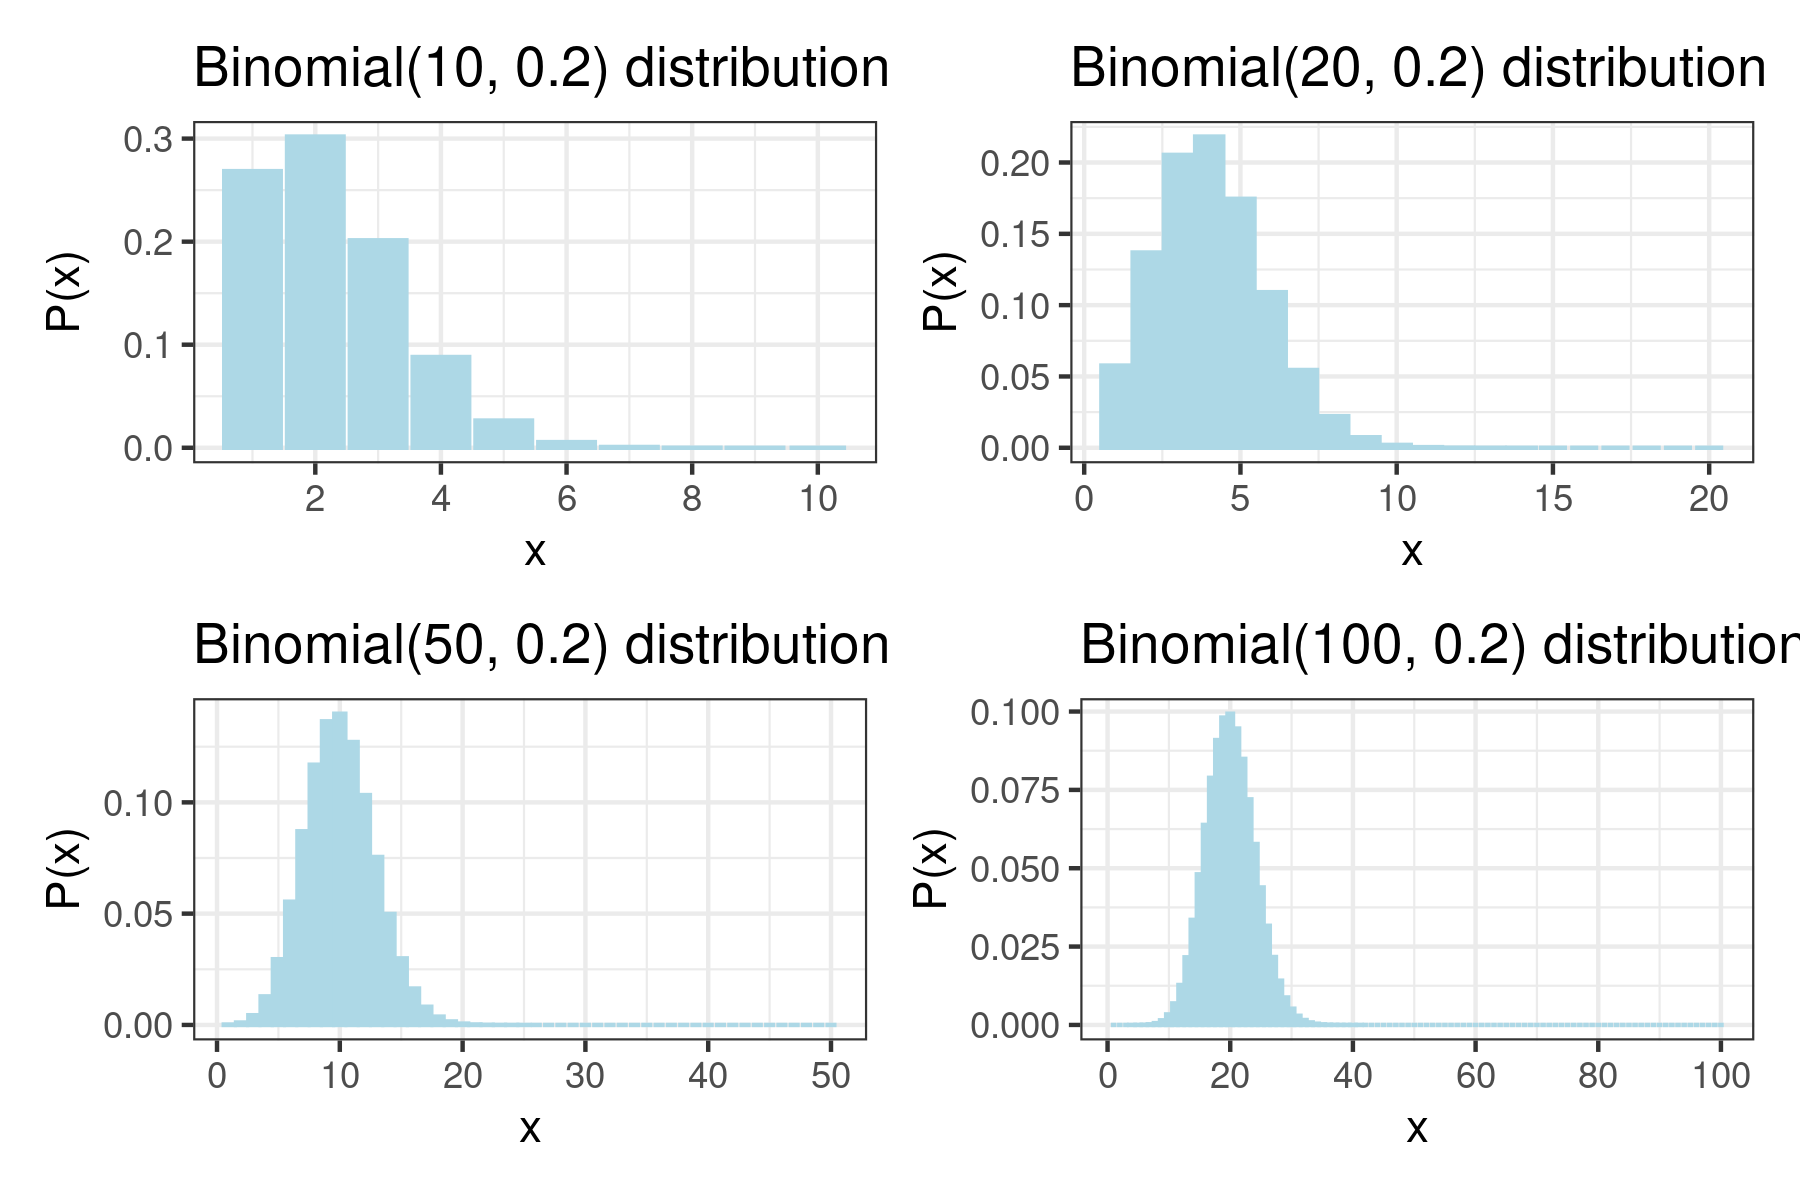
\includegraphics[width = 0.9\textwidth]{./figures/binomial_normal_approx.png}
  \caption{Biniomial distributions for $p$ fixed at
  $p = 0.2$ while $n$ varies. }
  \label{fig:norm_approx}
\end{figure}

What do you notice about the Binomial distributions
in Figure~\ref{fig:norm_approx}?


\fbox{\begin{minipage}{\textwidth}
{\bf The normal approximation
to the binomial distribution}.
Let $X$ be binomially distributed
with parameters $(n, p)$.
If $np(1 - p)$ is large, then
\begin{align*}
  \P(X\in [a, b]) \approx
  \int_{l}^u \frac{1}{\sqrt{2\pi\sigma^2}}
  \exp^{-\frac{1}{2\sigma^2}(x - \mu)^2} \; dx,
\end{align*}
where
\begin{itemize}
  \item $\mu = np$
  \item $\sigma^2 = np(1 - p)$
  \item $l = {a - \mu - 0.5}{\sigma}$
  \item $u = {b - \mu + 0.5}{\sigma}$.
\end{itemize}
In other words, $X$ is approximately follows a
normal distribution with mean $\mu = np$ and variance $\sigma^2 = np(1 - p)$.
\end{minipage}}

Note: the extra $\pm 0.5$ is called the continuity correction, and helps make better approximations.
It does not make a big difference, unless $a$ and $b$ are close.

\begin{exercise}[Airline overbooking]
  An airline estimates that about 90\% of passengers
  who reserve seats will show up for their flight.
   On a particular flight with 300 seats,
   the airline accepts 324 reservations.
   Assume all passengers show up independently of each other. Use the normal approximation to the binomial distribution
   to compute the probability that the flight will be
   overboooked.
\end{exercise}

\subsection{Confidence intervals}

The normal approximation above allows us to
construct confidence intervals. As a concrete example,
suppose we want to estimate the proportion of voters
in the United States
who will vote for the Democratic Party in the
upcoming election.
Let $p$ be the proportion of registered voters
who will vote Democratic.

The true proportion $p$ is an unknown quantity
that we would like to estimate. To form an estimate, we
randomly subsample $n = 200$ individuals
from the set of all registered voters and ask
about their voting preferences.
Suppose that in the sample, $110$ out of the $200$
individuals responded that they would vote
Democratic.
Let us estimate $p$ with $\hat p = 110/200 = 0.55$.
How good is the estimate $\hat p$?

We use the normal approximation to
construct a confidence interval using the following steps:
\begin{enumerate}
  \item We model the number of Democratic respondents as
  $n\hat p \sim \text{Binomial}(n, p)$.
  In our polling example, $n = 200$, $n\hat p = 110$, and $p$ is unknown.
  \item Using the normal approximation, we make the simplification that
  $n\hat p \sim \text{Normal}(np, np(1-p))$.
  \item By the shifting and scaling properties
  of a Normal,
  observe that
  \begin{align*}
    Z = \frac{n\hat p - np}{\sqrt{np(1-p)}} \sim \text{Normal}(0, 1).
  \end{align*}
  \item For a standard normal variable, note that
  \begin{align*}
    \P(-1.96 \leq Z \leq 1.96) = 0.95.
  \end{align*}
  \item Plug in our definition of $Z$, and re-arrange:
  \begin{align}
    \P\left(-1.96 \leq \frac{n\hat p - np}{\sqrt{np(1-p)}} \leq 1.96\right) &= 0.95.
    \iff \\
    \P\left(\hat p -1.96\sqrt{\frac{p(1-p)}{n}} \leq p \leq \hat p + 1.96\sqrt{\frac{p(1-p)}{n}}\right) &= 0.95
    \label{eq:pivot}
  \end{align}
  \item The above display \ref{eq:pivot} says that the interval
  \begin{align}
    \Big[\hat p - 1.96\sqrt{\frac{p(1-p)}{n}} \;,\;
    \hat p + 1.96\sqrt{\frac{p(1-p)}{n}}\Big]
    \label{eq:ci_truth}
  \end{align}
  will cover the true, unknown $p$ with probability 0.95.

  However, the formula \ref{eq:ci_truth} still depends on the unknown $p$.
  We plug in $\hat p$ for $p$ to construct our final confidence interval,
  \begin{align*}
    \Big[\hat p - 1.96\sqrt{\frac{\hat p(1-\hat p)}{n}} \;,\;
    \hat p + 1.96\sqrt{\frac{\hat p(1-\hat p)}{n}}\Big]
  \end{align*}
\end{enumerate}

Applying this formula to our polling example with $\hat p = 0.55$ and $n = 200$, our confidence interval is
$[0.51, 0.59]$.

Discussion: why is the Binomial model in step 1 appropriate here? In what scenarios might it be inappropriate?

\subsection{Central limit theorem}
The normal approximation is not limited to Binomial distributions.
More generally, we have

\fbox{\begin{minipage}{\textwidth}
{\bf The central limit theorem}. Suppose $X_1, ..., X_n \stackrel{iid}{\sim} F$.
Let $\mu = \E(X_1)$, be the mean of the distribution $F$
and $\sigma^2 = \V(X_1)$ be its variance.
Assume $\sigma^2 < \infty$. Then the random variable
%
\begin{align*}
  Z = \frac{\bar X_n - \mu}{\sigma / \sqrt{n}}
\end{align*}
is approximately $\text{Normal}(0, 1)$ distributed.
In other words
\begin{align*}
\P(Z\in[a, b])\approx \int_{a}^b
\frac{1}{\sqrt{2\pi}}
\exp^{-\frac{1}{2}x^2} \; dx,
\end{align*}
for all $a\leq b\in \R$.

\end{minipage}}

\begin{exercise}[CLT-based confidence intervals]
Suppose I want to know if a certain GRE prep course
actually improves GRE scores for participants.
I select a sample of 50 students who took this course,
and for each student, I compute their difference in scores
before and after the course.
The sample average of these differences
was +5, with a sample standard deviation of 8.

\begin{enumerate}[label = (\alph*)]
  \item Use the central limit theorem to construct a 95\% confidence interval for the change in GRE scores.
  \item Is there statistical evidence that students
  perform better on GRE at the end of this course?
  \item Can we conclude that this GRE course is helpful for students? Why or why not?
\end{enumerate}

\end{exercise}

\section{Poisson approximation}

In the section above, we saw that if $np(1-p)$ is large,
then a normal distribution can be used to approximate
the binomial distribution.
However, the normal approximation will not be appropriate
if $1/p$ is on the same order of magnitude as $n$.
See Figure~\ref{fig:pois_approx}.
Do you see above why the normal approximation is not
appropriate here?


\begin{figure}[!h]
  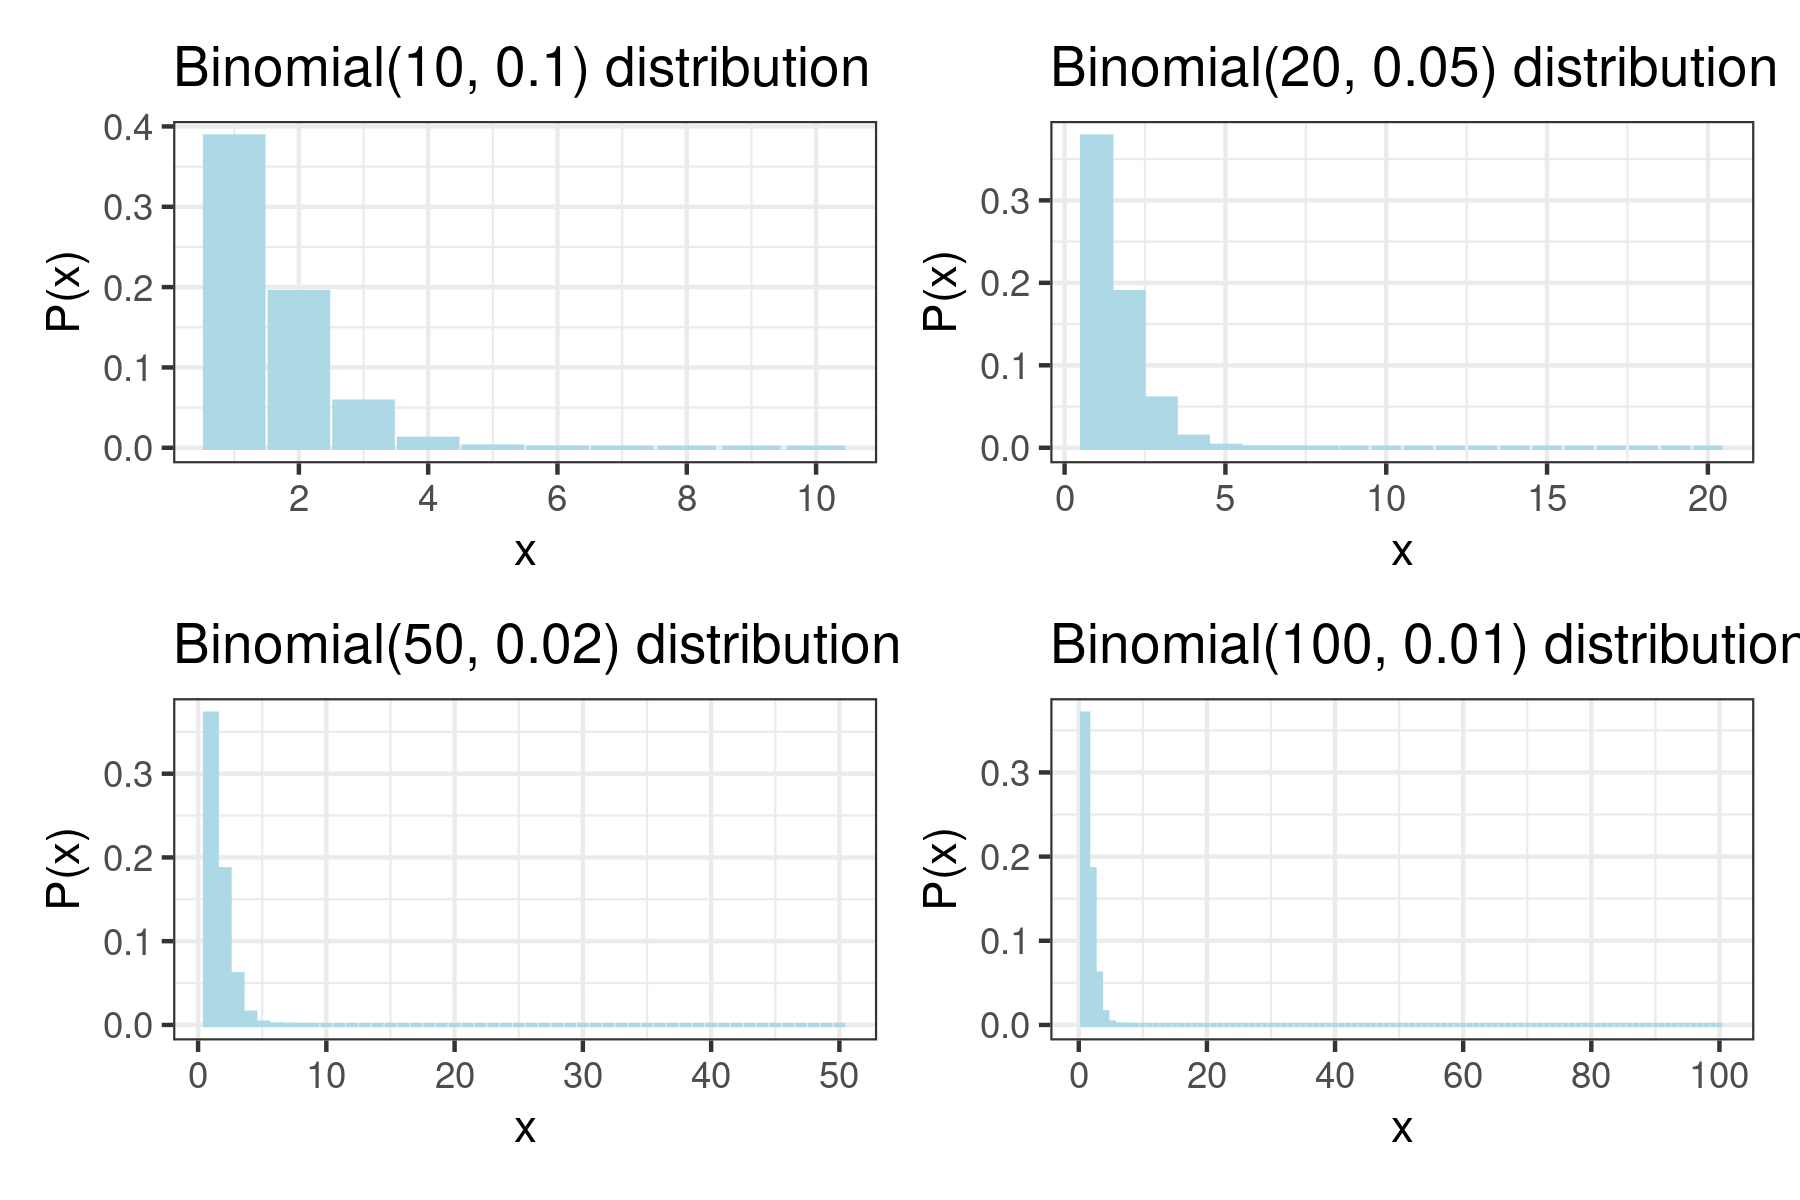
\includegraphics[width = 0.9\textwidth]{./figures/binomial_poisson_approx.png}
  \caption{Biniomial distributions for $np$ fixed at $np = 1$, while $n$ varies. }
  \label{fig:pois_approx}
\end{figure}

A more appropriate approximation in such scenarios
is the Poisson
distribution.

\fbox{\begin{minipage}{\textwidth}
{\bf The Poisson approximation to the binomial distribution}.
Let $X$ be binomially distributed with
parameters $(n, p)$.
If $n$ is large and $p$ is small, then
$X$ is approximately Poisson distributed
with mean $\lambda = np$.
That is,

\begin{align*}
  \P(X = k) \approx \exp^{-\lambda}\frac{\lambda^k}{k!}
\end{align*}

\end{minipage}}

In particular, the approximation becomes exact as $n\rightarrow \infty$ with $p = \lambda / n$.

This is sometimes called the ``law of small
numbers" or the ``law of rare events,"
since convergence happens as $p$ gets small
with increasing $n$.

\begin{example}[Raindrops in a bucket]
  I place a bucket outside in a rainstorm.
  The number of raindrops falling in my bucket
  is well-modeled with a Poisson distribution.
  The total number of raindrops $n$ falling from the sky
  is large, but the probability $p$ of any raindrop falling in my bucket is small.
\end{example}

\begin{exercise}[]
Suppose that a manufactoring process has a
1\% chance of producing a defective item.
Use the Poisson approximation to compute the probability
that in a batch of 200 items, there are two or more
defective items.
\end{exercise}

\subsection{Poisson arrivals}

The Poisson distribution is often used to model the number
of occurences of some event during an interval of time.
Examples include:
\begin{itemize}
  \item The number of car accidents at an
   intersection in a given week.
  \item The number of earthquakes occuring in the Bay Area in a given month.
  \item The number of customers arriving at a coffee shop between noon and 1pm.
\end{itemize}

In this subsection, we will use the Poisson approximation
to the binomial to justify why (or why not) the
Poisson distribution is appropriate in these examples.

For concreteness, let us take the last example, the number
of arrivals at a coffee shop.
Suppose from historical data, we observe that on average,
$\lambda = 30$ customers arrive between noon and 1pm.

To see why the Poisson distribution may be a good model
for th number of arrivals,
divide the time between noon and 1pm into $(1/n)$-hour
intervals. Then, assume
\begin{itemize}
  \item At most one arrival can occur during any
  $(1/n)$-hour interval.
  \item Whether or not an arrival occurs during a
  $(1/n)$-hour interval happens with probability $\lambda / n$.
  \item The occurance of arrivals in each interval is independent of all other intervals.
\end{itemize}

With the above assumptions, the total number of arrivals
in a one-hour period is distributed as
$\text{Binomial}(n, \lambda / n)$ (do you see why?).

Taking $n\rightarrow\infty$, the law of rare events
states that the number
of arrivals is Poisson with mean $\lambda$.

\textbf{So when are these assumptions appropriate?} The first is
mostly non-controversial,
since the intervals get smaller and smaller as  $n\rightarrow\infty$.
The second says that the \textit{rate of arrivals are constant} in this one-hour interval.
This assumption would not be met if, for example, there is a large undergraduate lecture that ends at 12:30pm, resulting in a surge of customers at 12:35pm.
The last assumption says that \textit{arrivals must be independent} -- this assumption would not be met if,
for example, customers tend to arrive in pairs or groups.

This does not mean that the Poisson distribution is useless as a model for the world.
Often, these simple distributions form the building blocks for more complex models. We start with simple model
and iteratively refine them, either by incorporating
domain expertise or by employing data driven algorithms.
All model building exercises depend on careful analysis of the assumptions --
and these assumptions may be rejected based on either
domain knowledge or observed data.

\subsection{Arrival times}

\begin{exercise}[Arrival times]
Often, we are interested not only in the number of arrivals,
but also when these arrivals occur.
Show that if the number of arrivals in $t$-units of time
follows a Poisson distribution with mean $\lambda t$,
then the \textit{time} of the first arrival
has an exponential distribution with rate $\lambda$.

\end{exercise}


In fact, if we further assume that the number of arrivals in
disjoint time intervals are independent, then
the arrival times follow a \textit{Poisson process},
in which case the time between any two arrivals will be exponentially distributed.


\fbox{\begin{minipage}{\textwidth}
\textbf{Two descriptions of Poisson arrivals}.
The following describes equivalent processes:

\begin{enumerate}[label = (\Roman*)]
  \item The \textit{number of arrivals} in an interval time of length $t$ is
  $\text{Poisson}(\lambda t)$, and the number of arrivals in disjoint
  time intervals are independent.

  \item The \textit{time between arrivals}
  are independent and distributed as $\text{Exponential}(\lambda)$.
\end{enumerate}

\end{minipage}}

\begin{exercise}[Arrivals at a coffee shop]
Suppose customers arrive at a coffee shop at an average, time-invariant
rate of 12 customers per hour according to a Poisson arrival process.
%
% Let $N(t_1, t_2)$ be the random variable representing the number of arriving customers
% between times $t_1$ and $t_2$.
% Fro concreteness, let $t = 0$ refer to 8am, while $t > 0$ refers to
% the number of hours elapsed after 8am.
%
% Let $W_1$ be the time of the first arrival after 8am, and let
% $W_i$ for $i > 1$ be the time between subsequent arrivals.
%
Compute

\begin{enumerate}[label = (\alph*)]
  \item The probability that no one arrives between 8am and 8:30am.
  \item The probaiblity that no one arrives between 8 and 8:30am,
  and at most four people arrive between 8:30 and 9am.
  \item The probability that the fourth customer arrives within 10 minutes
  of the third customer.
  \item The probability that the first arrival takes less than 10 minutes
  while the time between the second and third arrival is more than 30 minutes.
  \item The probability that the 10th customer takes more than an hour to arrive.
\end{enumerate}

\end{exercise}



\end{document}
